Detektiranje rubova može se promatrati kao tehnika čitanja rubova objekata vidljivih na slici.
Samo po sebi jedna je od osnovnih, nisko razinskih tehnika računalnog vida s mnogim primjenama visoke razine, uključujući detekciju objekata i segmentaciju slike (\emph{eng. Image Segmentation}) (\cite{Liu_2019}).

Problem je definiran kao pokušaj imitiranja rada \emph{Sobel} operatora.

 \paragraph{Sobel operator} također je operator koji koristi konvoluciju.
 Koriste se dvije konvolucijske jezgre (\cite{Sekanina2011}):
 \[
	 p = \frac{1}{8}
	 \begin{bmatrix}
		 -1 && 0 && 1 \\
		 -2 && 0 && 2 \\
		 -1 && 0 && 1
	 \end{bmatrix}
	 ,\ 
	 q = \frac{1}{8}
	 \begin{bmatrix}
		 -1 && -2 && -1 \\
		 0 && 0 && 0 \\
		 1 && 2 && 1
	 \end{bmatrix}
 \]
Zajedno, jezgre služe kako bi se izračunao gradijent slike.
Jezgra $p$ koristi se kako bi se izračunala procjena derivacije za horizontalne promjene, a $q$ za vertikalne. \\
Vrijednost novonastale slike $G$ na koordinatima $(i, j)$ računa se kao
$$
G_{(i, j)} = c + |p_{(i, j)}| + |q_{(i, j)}|
$$
gdje je $c$ proizvoljna konstanta, npr. $c = 128$.
Primjer djelovanja Sobel operatora na fotografiju Lene vidljiv je na slici \ref{fig:lena_sobel}.

\begin{figure}
	\centering
	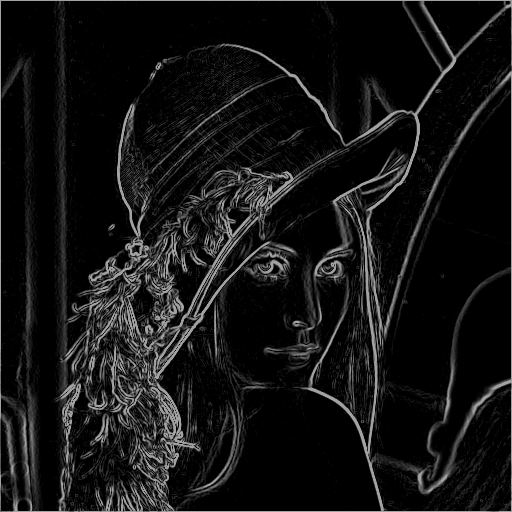
\includegraphics[width=0.6\linewidth]{Experiments/EdgeDetection/lena_sobel.png}
	\caption{Primjer djelovanja Sobel operatora na fotografiju Lene}
	\label{fig:lena_sobel}
\end{figure}

\subsubsection{Postavke}
Za razliku od micanja šuma koristi se konvolucijska jezgra koja prihvaća i srednju promatranu vrijednost.
Time, filter možemo definirati kao $f(x): [0, 255]^9 \rightarrow [0, 255]$.

Fotografije koje su se promatrale u trening i validacijskoj fazi vidljive su na slici \ref{fig:edge_detection_train_val_in}.
Umjesto direktne usporedbe sa Sobel slikama, odlučio sam se na usporedbu sa slikama dobivenim \emph{Canny} algoritmom.
Slike nastale primjenom Canny algoritma imaju vrijednosti $0$ ili $1$ ovisno pripada li promatrana vrijednost na koordinatama $(i, j)$ rubu što sam koristio kao prednost u razvoju modela.
Jednako kao u više-kategoričkoj klasifikaciji gdje se koristi vektor vrijednosti gdje su sve vrijednosti $0$ osim točne koja je $1$ (\emph{eng. One Hot Encoding}).

\begin{figure}
	\centering
	\caption{Fotografije Lene i Kamermana nakon primjene detekcije ruba \emph{Canny} algoritmom}
	\begin{subfigure}[t]{0.45\textwidth}
		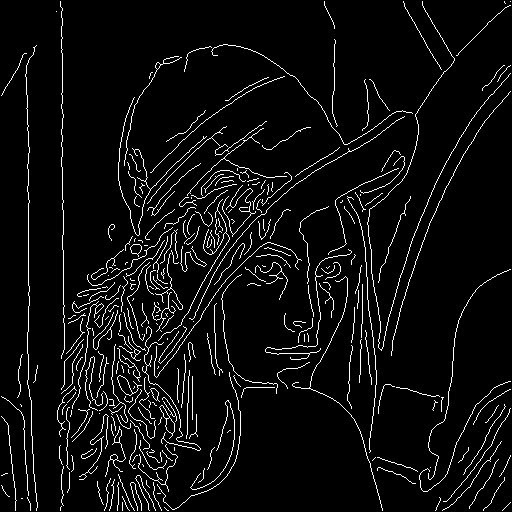
\includegraphics[width=\textwidth]{Experiments/EdgeDetection/lena_canny.jpg}
		\caption{Lena nakon primjene Canny filtera}
		\label{fig:lena_canny}
	\end{subfigure}
	\begin{subfigure}[t]{0.45\textwidth}
		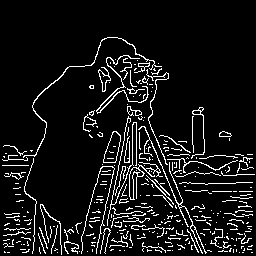
\includegraphics[width=\textwidth]{Experiments/EdgeDetection/cameraman_canny.jpg}
		\caption{Kamerman nakon primjene Canny filtera}
		\label{fig:camerman_canny}
	\end{subfigure}
	\label{fig:edge_detection_train_val_in}
\end{figure}

Problem koji se rano javio je što je $\approx 70\%$ slike vrijednosti $0$, odnosno, crno.
Rezultat toga i korištenja $L1$ pogreške je navođenje modela da teži samo predviđanju te vrijednosti.
Korištenje srednje kvadratne pogreške (\emph{eng. Mean Squared Error (MSE)})
$$err = \frac{1}{n}\sum_{i=1}^{n}(y_{cgp} - y_{skup\ podataka})^2$$
pokazalo se dobrim rješenjem.
U slučaju veće razlike npr. predviđanje $1$ na željenu vrijednost $0$ unutar sume rezultiralo bi razlikom od $255^2$, dok bi manje razlike težile ka $0$.

Tablica \ref{table:edge_detection_function_set} prikazuje funkcije koje su se mogle koristiti u čvorovima.
Vrijednosti nisu morale biti unutar skupa $[0, 255]$, a na izlazu bi se prilagodile najbližoj rubnoj vrijednosti u slučaju da izlaz nije unutar skupa.
Također, ako se funkciji $3$, dijeljenju, prosljedi nepodržana vrijednost u nazivnik, funkcija se koristi kao funkcija identiteta, odnosno $f(x, y) = x$.
Algoritam odabira je $1 + \lambda$ s $\lambda = 8$.
Povećanje parametra $\lambda$ zahtjeva smanjenje najvećeg dozvoljenog broja iteracija koji je postavljen na $20$, puno manje nego pri micanju šuma gdje je definirano kao $500$.

\begin{table}
	\centering
	\begin{tabular}{||c c c c||}
		\hline
		Adresa funkcije & Funkcija & Broj ulaza & Broj izlaza\\ [0.5ex]
		\hline \hline
		0 & $x + y$ & 2 & 1\\
		1 & $x - y$ & 2 & 1\\
		2 & $x \cdot y$ & 2 & 1\\
		3 & $\frac{x}{y}$ & 2 & 1 \\
		4 & $\sqrt{x}$ & 1 & 1\\
		5 & $avg$ & 9 & 1\\
		6 & $min$ & 9 & 1\\
		7 & $max$ & 9 & 1\\
		8 & $\ln(x)$ & 1 & 1\\
		9 & $\sin(x)$ & 1 & 1\\
		10 & $\cos(x)$ & 1 & 1\\
		11 & $step(x)$ & 1 & 1\\ [1ex]
		\hline
	\end{tabular}
	\caption{Funkcije korištene pri detekciji rubova}
	\label{table:edge_detection_function_set}
\end{table}

Promatrani podskupovi veličina su $40 \times 40$.
Time, skup podataka sastoji se od $1600$ vektora ($|v| = 9$), po jedan za svaku promatranu konvolucijsku jezgru.
Trening i validacijski skup uzet je sa iste fotografije Lene u dva odvojena podskupa (\ref{fig:edge_detection_in_out_pair_example}), dok je za testnu fotografiju odabrana fotografija kamermana.

\begin{figure}
	\centering
	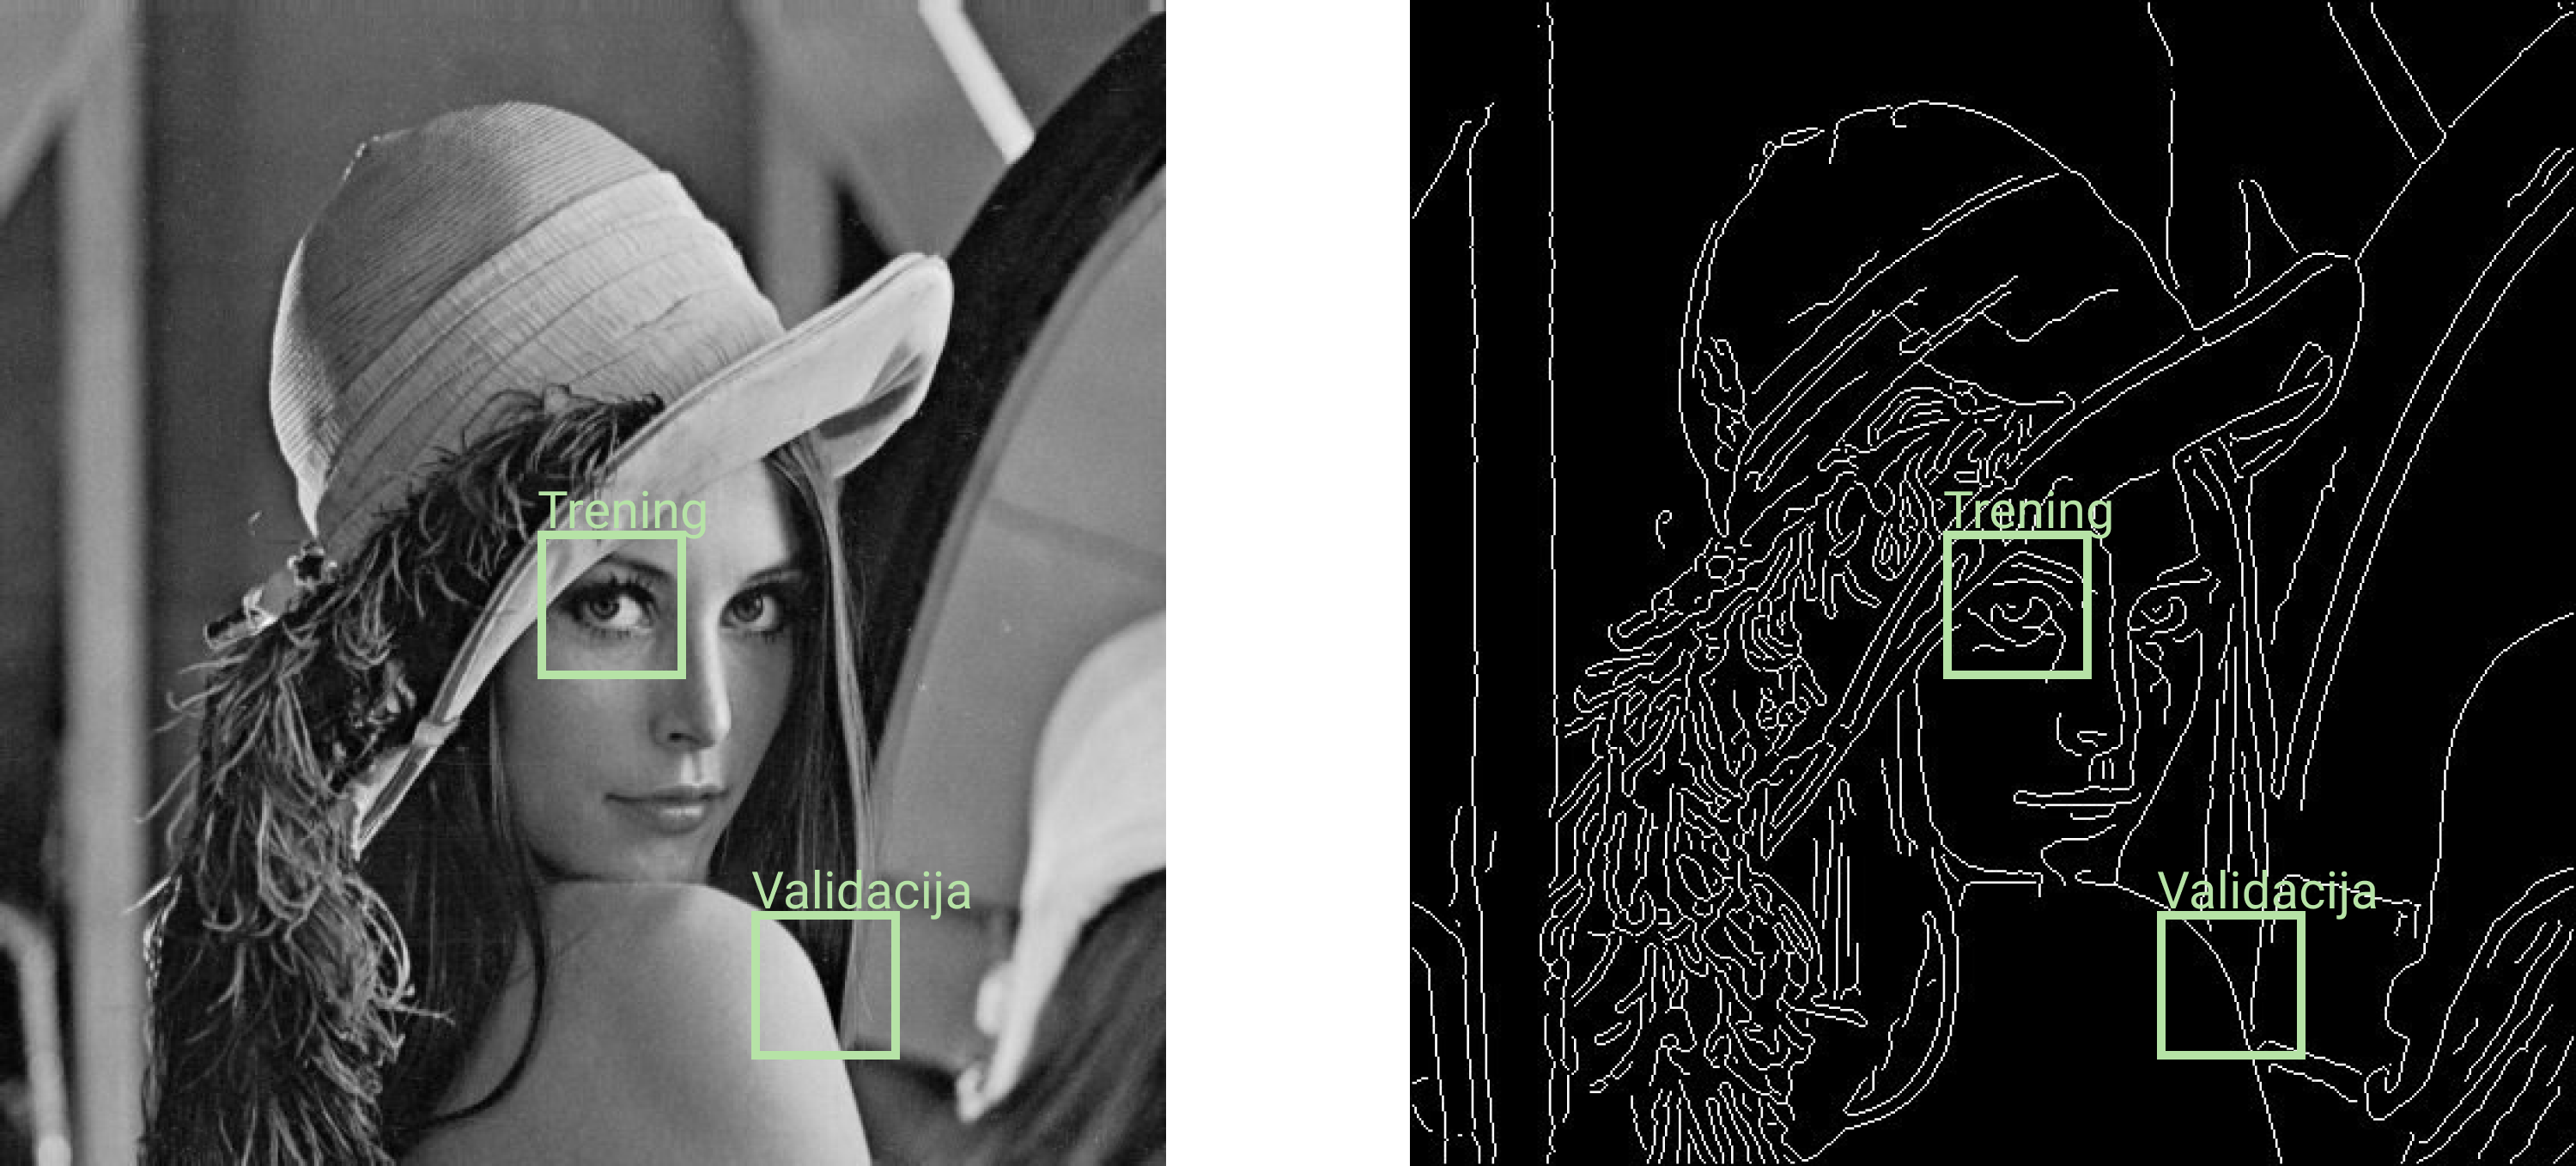
\includegraphics[width=\linewidth]{Experiments/EdgeDetection/edge_detection_in_out_pair.png}
	\caption{Ulazna i željena izlazna slika za detekciju ruba s označenim podskupovima za trening i validaciju}
	\label{fig:edge_detection_in_out_pair_example}
\end{figure}

\subsubsection{Rezultati}
Rezultati detekcije ruba vidljivi su na slikama \ref{fig:edge_detection_results}. % TODO: Dodati graf!
Pomalo neočekivano, rezultati izgledaju bolje na testnoj slici, no to pridodajem značajkama fotografije pogodnijim za detekciju rubova.
Zbog toga, vjerujem da je dosta težak zadatak za detekciju rubova fotografija s vidljivom kosom ili bilo kakvim sitnim detaljima.
Veliku ulogu igrao je i izbor podskupa iz kojeg se isčitavaju podaci za trening.
Količina praznog dijela, vrsta i broj vidljivih krivulja, zajedno s ispravnim odabirom funkcije koju minimiziramo igra najveću ulogu.
U usporedbi s problemom micanja šuma, detekcija rubova rješenje pronalazi iznimno brzo.
Svako pokretanje koje je završilo s uspješnim pronalaskom rješenja konvergiralo je u $\leq 10$ iteracija.

\begin{figure}
	\centering
	\caption{Fotografije Lene i Kamermana prije i nakon detekcije rubova}
	\begin{subfigure}[t]{0.48\textwidth}
		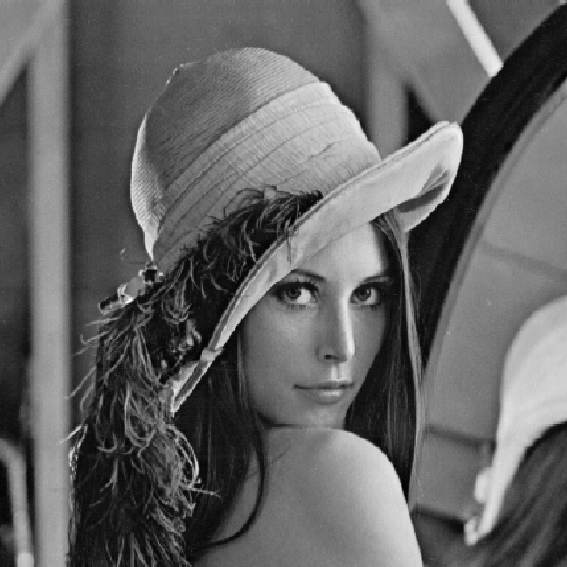
\includegraphics[width=\textwidth]{Experiments/GrainRemoval/lena.png}
	\end{subfigure}
	\begin{subfigure}[t]{0.48\textwidth}
		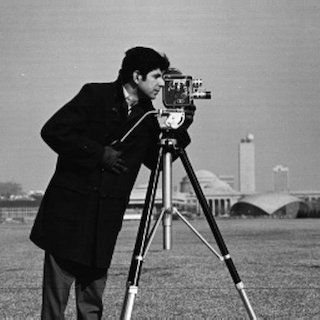
\includegraphics[width=\textwidth]{Experiments/GrainRemoval/cameraman.jpg}
	\end{subfigure}
	\begin{subfigure}[t]{0.48\textwidth}
		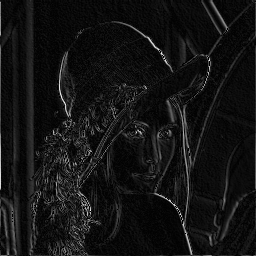
\includegraphics[width=\textwidth]{Experiments/EdgeDetection/lena_edges.png}
	\end{subfigure}
	\begin{subfigure}[t]{0.48\textwidth}
		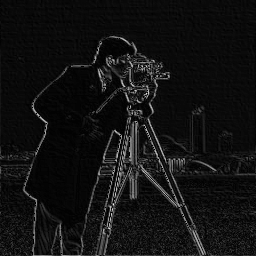
\includegraphics[width=\textwidth]{Experiments/EdgeDetection/camerman_edges.png}
	\end{subfigure}
	\label{fig:edge_detection_results}
\end{figure}

Graf \ref{fig:edge_detection_graph} pokazuje kretanje pogreške na trening i validacijskom skupu podataka.
Greška se čini niska već pri pokretanju no to je zbog prirode algoritma.
Iz početnog stvaranja potencijalnog roditelja kao najbolji odabire se najčešće onaj koji veliku večinu rezultata računa kao $0$ što je u svakom slučaju točno za većinu skupa podataka.
Daljni koraci vrlo brzo konvergiraju točnijim rješenjima.

\begin{figure}
	\centering
	\caption{\emph{MSE} pogreška na trening i validacijskom skupu kroz iteracije algoritma}
	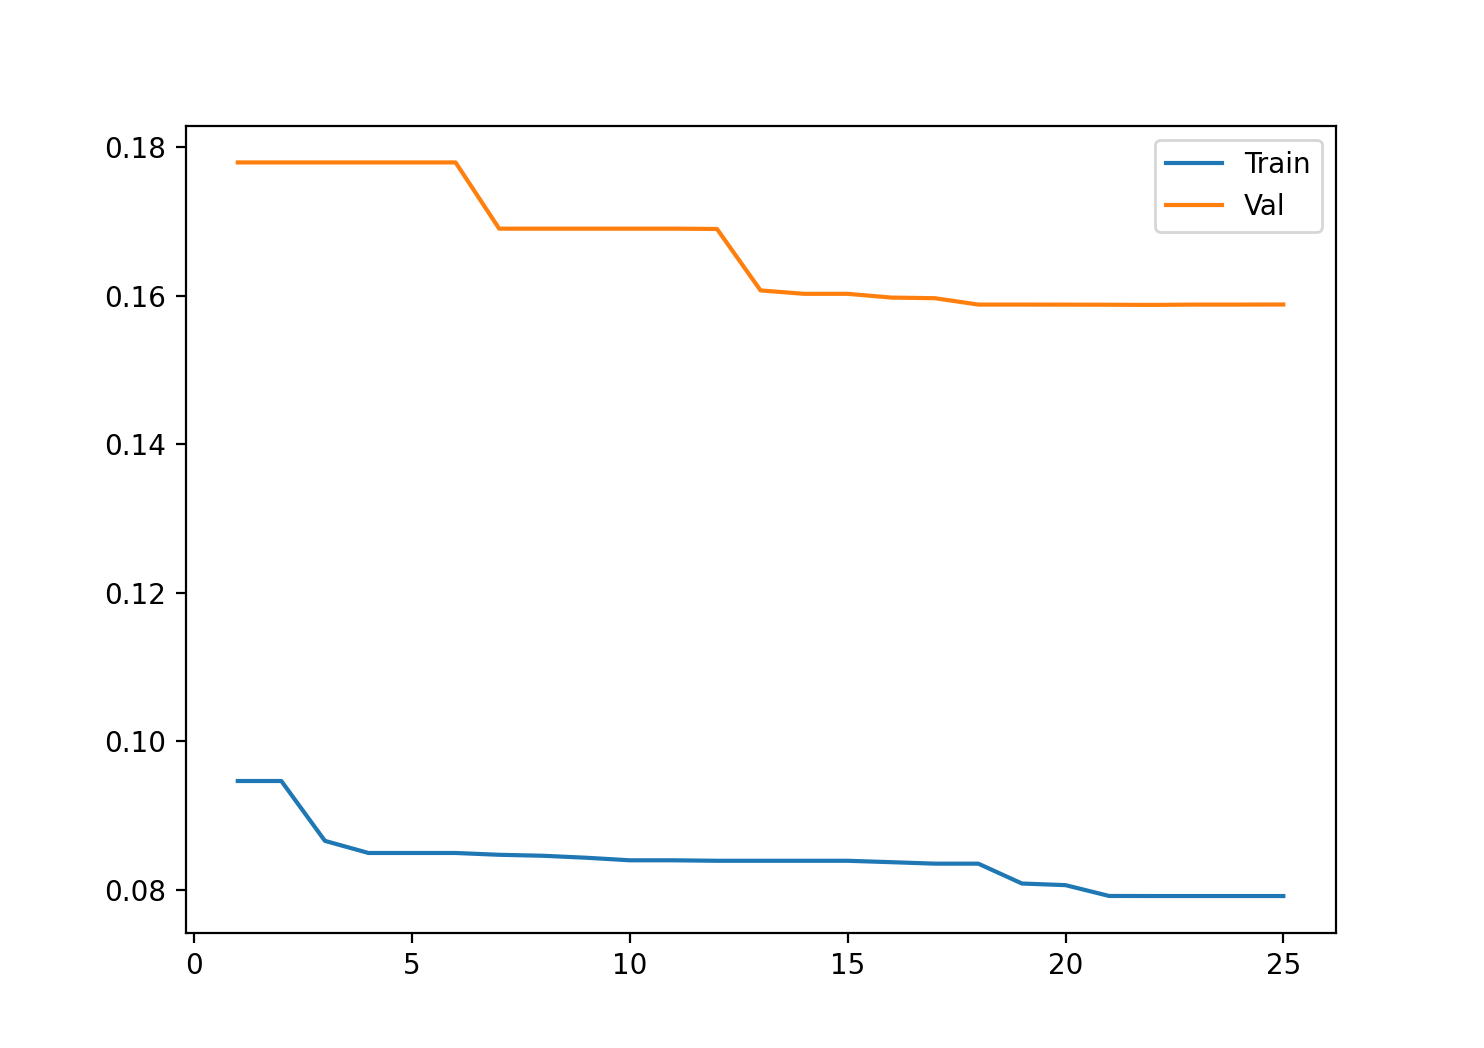
\includegraphics[width=0.6\linewidth]{Experiments/EdgeDetection/edge_detection_graph.png}
	\label{fig:edge_detection_graph}
\end{figure}
